\section{Introduction}
	
	Despite its significance in nature, the brain is one of the least understood
	entities known to science. Current attempts to understand the brain centre on
	building models of its behaviour. Though models such as Spaun are able to
	produce high-level, realistic behaviour, they run slowly with conventional
	computers taking 2.5 hours to simulate one second of neural activity
	\cite{eliasmith12}.
	
	Neural models are typically a large graph of `neurons' each being connected to
	potentially thousands of others. Signals, known as spikes, are produced by
	each neuron at an average rate of 10 Hz which each spike being destined for
	around 1,000 other neurons. With billions of neurons in a large neural model
	this results in very large numbers of very small messages being passed around
	the simulator \cite{vainbrand11}. Because neurons are often cheap to simulate,
	typical super computers featuring powerful processors with comparatively
	limited interconnection networks perform poorly.
	
	The Blue Brain project has built a model with extremely realistic neuron
	behaviour which can exploit typical super-computer resources \cite{markram06}.
	However, models are severely limited in size to hundreds of thousands of
	neurons compared with the 85 billion in a human brain. This work instead
	focuses on the simulation of large networks of simple neurons such as Spaun.
	
	Due to the unsuitability of conventional architectures, special-purpose
	systems have been built for neural simulation. In this short report, current
	attempts to overcome these limitations are described followed by an overview
	of preliminary work carried out on the SpiNNaker brain simulation
	architecture. The report concludes with the research plan proposed to develop
	this research eventually to yield an improved architecture for brain
	simulation with a focus on the topology of the interconnection network.

\section{Brain Simulators}
	
	Current special purpose brain-simulation architectures can be divided into two
	categories: those based on conventional digital circuits and those based on
	analogue electronics inspired by the analogue mechanisms in the brain. Though
	analogue systems can be very power efficient the maturity of digital design
	techniques has meant that modern analogue simulators are `mixed mode'
	implementing only the neurons using analogue electronics and interconnecting
	them with digital electronics. As a result, the interconnection networks of
	modern analogue and digital simulators are typically directly comparable.
	
	This section describes the interconnection network of three notable
	architectures. A wider and more detailed survey of current simulation
	architectures is available by Misra and Saha \cite{misra10}.
	
	\begin{figure}
		
		\center
		\begin{subfigure}[b]{0.32\textwidth}
			\center
			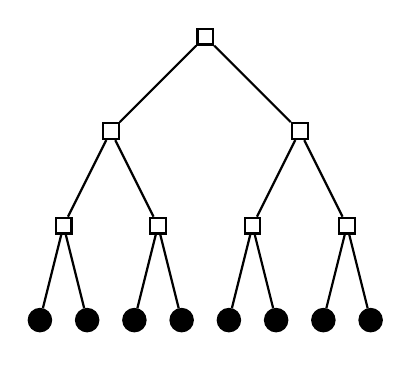
\begin{tikzpicture}[thick, node distance=1em,level distance=1.2cm]
	
	% Bodge/Hack to vertically center with mesh and torus figures.
	\draw [white] (-1.3cm,-3.85cm) rectangle ++(2cm,2cm);
	
	\begin{scope}[every node/.style={draw,rectangle,thick},             inner sep=0.1cm]
		\tikzstyle{level 1}=[sibling distance=2.4cm,every child/.style  ={},inner sep=0.1cm]
		\tikzstyle{level 2}=[sibling distance=1.2cm,every child/.style  ={},inner sep=0.1cm]
		\tikzstyle{level 3}=[sibling distance=0.6cm,every child/.style={},inner sep=0.1cm]
		
		\node {}
			child {node {}
				child {node {}
					child {node [fill,circle] {}}
					child {node [fill,circle] {}}
				}
				child {node {}
					child {node [fill,circle] {}}
					child {node [fill,circle] {}}
				}
			}
			child {node {}
				child {node {}
					child {node [fill,circle] {}}
					child {node [fill,circle] {}}
				}
				child {node {}
					child {node [fill,circle] {}}
					child {node [fill,circle] {}}
				}
			}
		;
	\end{scope}
	
\end{tikzpicture}


			\caption{Binary Tree}
			\label{fig:binary-tree}
		\end{subfigure}
		\begin{subfigure}[b]{0.32\textwidth}
			\center
			\begin{tikzpicture}[thick,inner sep=0.1cm,3d/perspective eye={0,10,20}]
	\def\width{5}
	\def\height{5}
	
	\def\tubewidth{1}
	\def\holesize{5}
	
	\pgfmathtruncatemacro{\widthh}{\width - 1}
	\pgfmathtruncatemacro{\heightt}{\height - 1}
	
	\clip (-0.7,-0.3) rectangle (\widthh+0.7,\heightt+0.7);
	
	\foreach \lx in {0,...,\widthh}{
		\foreach \ly in {0,...,\heightt}{
			\node [fill,circle]
			      (node X\lx Y\ly) at (\lx, \ly)
			      {};
		}
	}
	
	% Draw normal links
	\foreach \x in {0,...,\widthh}{
		\foreach \y in {0,...,\heightt}{
			\pgfmathtruncatemacro{\xx}{\x + 1}
			\pgfmathtruncatemacro{\yy}{\y + 1}
			\ifthenelse{\xx < \width}{
				\draw (node X\x Y\y.center) -- (node X\xx Y\y.center);
			}{
				%\draw (node X\x Y\y.center) -- (node X0Y\y.center);
			}
			\ifthenelse{\yy < \height}{
				\draw (node X\x Y\y.center) -- (node X\x Y\yy.center);
			}{
				%\draw (node X\x Y\y.center) -- (node X\x Y0.center);
			}
		}
	}
	
	% Draw Long Links
	% \begin{pgfonlayer}{background}
	% 	\foreach \x in {0,...,\widthh}{
	% 		\draw [help lines] (node X\x Y0.center)
	% 		            .. controls +(0.7,-2.0)
	% 		                    and +(0.7,2.0)
	% 		            .. (node X\x Y\heightt.center);
	% 	}
	% 	\foreach \y in {0,...,\heightt}{
	% 		\draw [help lines] (node X0Y\y.center)
	% 		            .. controls +(-2.0,0.7)
	% 		                    and +(2.0,0.7)
	% 		            .. (node X\widthh Y\y.center);
	% 	}
	% \end{pgfonlayer}
	
\end{tikzpicture}


			\caption{2D Mesh}
			\label{fig:mesh}
		\end{subfigure}
		\begin{subfigure}[b]{0.32\textwidth}
			\center
			\begin{tikzpicture}[thick,inner sep=0.1cm,3d/perspective eye={0,10,20}]
	\def\width{5}
	\def\height{5}
	
	\def\tubewidth{1}
	\def\holesize{5}
	
	\pgfmathtruncatemacro{\widthh}{\width - 1}
	\pgfmathtruncatemacro{\heightt}{\height - 1}
	
	\clip (-0.7,-0.3) rectangle (\widthh+0.7,\heightt+0.7);
	
	\foreach \lx in {0,...,\widthh}{
		\foreach \ly in {0,...,\heightt}{
			\node [fill,circle]
			      (node X\lx Y\ly) at (\lx, \ly)
			      {};
		}
	}
	
	% Draw normal links
	\foreach \x in {0,...,\widthh}{
		\foreach \y in {0,...,\heightt}{
			\pgfmathtruncatemacro{\xx}{\x + 1}
			\pgfmathtruncatemacro{\yy}{\y + 1}
			\ifthenelse{\xx < \width}{
				\draw (node X\x Y\y.center) -- (node X\xx Y\y.center);
			}{
				%\draw (node X\x Y\y.center) -- (node X0Y\y.center);
			}
			\ifthenelse{\yy < \height}{
				\draw (node X\x Y\y.center) -- (node X\x Y\yy.center);
			}{
				%\draw (node X\x Y\y.center) -- (node X\x Y0.center);
			}
		}
	}
	
	% Draw Long Links
	\begin{pgfonlayer}{background}
		\foreach \x in {0,...,\widthh}{
			\draw  (node X\x Y0.center)
			            .. controls +(0.5,-1.8)
			                    and +(0.5,1.8)
			            .. (node X\x Y\heightt.center);
		}
		\foreach \y in {0,...,\heightt}{
			\draw  (node X0Y\y.center)
			            .. controls +(-1.8,0.5)
			                    and +(1.8,0.5)
			            .. (node X\widthh Y\y.center);
		}
	\end{pgfonlayer}
	
\end{tikzpicture}


			\caption{2D Torus}
			\label{fig:torus}
		\end{subfigure}
		
		\caption{Network topology examples. Dots represent chips, boxes represent
		switches which forward messages but perform no other computation.}
		\label{fig:network-topology-examples}
		
	\end{figure}
	
	\subsection{Neurogrid}
		
		The Neurogrid architecture consists of chips with analogue hardware to
		simulate tens of thousands of neurons. Spikes from these neurons are output
		by the chip serially and must be routed to each of the target neurons which
		may reside in other chips. Current prototypes feature 16 chips which form
		the leaves of a binary tree (figure \ref{fig:binary-tree}). This
		architecture can simulate around a million neurons with 100,000 times less
		power than a conventional super-computer \cite{choudhary12}.
		
		The binary tree interconnection network topology is scalable with network
		latency, in the ideal case, increasing $O(\log{N})$ with the number of
		chips. For neural simulation, however, tree topologies have been shown by
		Vainbrand and Ginosar to be non-optimal requiring large amounts of hardware
		to achieve the bandwidth required to transmit large numbers of spikes
		between nodes \cite{vainbrand11}.
	
	\subsection{BrainScaleS}
	
		The BrainScaleS project has developed an architecture which,
		unconventionally, uses an entire silicon wafer on which tens of chips have
		been produced side-by-side. Each chip contains a number of analogue neuron
		simulators which are interconnected via a 2D mesh network (figure
		\ref{fig:mesh}).  Spikes can be forwarded from chip to chip until they reach
		their destination \cite{schemmel08}. It is intended that multiple wafers
		will be combined with conventional Internet Protocol (IP) switches.
		
		Though mesh networks are easily scaled in principle, the BrainScaleS
		architecture is limited by the maximum size of a silicon wafer. The topology
		to be used to connect wafers together has not yet been decided.  Since
		silicon wafers are circular this means that the mesh networks on a wafer
		don't tessellate. Since gaps will be left in the network this may detract
		from the system's performance.
	
	\subsection{SpiNNaker}
	
		% Finally, the focus of my work so far: SpiNNaker has many small processors
		% connected via a torus network whose size is only limited by the address
		% space available to neurons. Network optimised for small (maybe zero-data)
		% packets.  Unlike the first two it runs simulations in software making it far
		% more flexible, easier with current understanding of electronics but less
		% power efficient.
		% 
		% Here's how it looks in implemented hardware: cores, chips and boards.
		
		The SpiNNaker architecture is a completely digital simulator which uses a
		large number of small, low-power general purpose processors \cite{furber06}. Eighteen
		processors are combined into chips which are connected in a toroid network.
		A toroid is a generalisation of a torus (figure \ref{fig:torus}) with chips
		connecting to more than four other chips as in figure \ref{fig:toroid}. This
		type of network was found to be optimal amongst common network topologies by
		Vainbrand and Ginosar for neural simulations \cite{vainbrand11}. This
		topology is easily scaled to arbitrary sizes by adding chips and is only
		limited by the number of bits used to address neurons in the system.
		
		\begin{figure}
			\center
			\input{figures/toroid}
			\caption{Section of the toroid topology used by SpiNNaker. Wrap-around
			links omitted.}
			\label{fig:toroid}
		\end{figure}
		
		Preliminary work, however, has found that further improvements can be made
		over torus-like topologies for use in neural simulation and this is
		described in the next section.

\section{Preliminary Work}
	
	Current work has focused on the SpiNNaker architecture and its interconnection
	network. This section outlines the work completed so far.
	
	\subsection{SpiNNaker Simulation}
		
		SpiNNaker systems are built by combining groups of 48 chips onto circuit
		boards which are then connected together via cables with the largest planned
		system containing 1,200 boards. Connections between chips on the same board
		use a low-cost technology using 16 wires. Connections between chips on
		different boards would require cables containing 768 wires which would be
		prohibitively expensive. Instead these board-to-board connections use more
		complex high-speed serial signalling which requires only 24 wires provided
		by commodity cables.
		
		A network interconnect simulator was developed which models the behaviour of
		the different kinds of link in a SpiNNaker system. The model showed that the
		use of high-speed serial links between boards increased the latency of
		spikes in the system by 80.4\%. High-accuracy neural simulations require
		that spikes are delivered with low latency and may suffer as a result of
		this increased latency. Though the models currently planned for use on
		SpiNNaker are coarser-grained, this latency penalty may pose a problem for
		future networks.
	
	\subsection{SpiNNaker Wiring}
	
		Large SpiNNaker machines will be constructed by placing boards into standard
		computer cabinets and with cables connecting them together. There are two
		key constraints which must be considered when deciding how to connect the
		boards together. Firstly, the high-speed signalling technology requires that
		the cables used be short, disallowing connections between cabinets at
		opposite ends of the system. Secondly, since the cables must be manually
		connected, the system must be simple to assemble.
		
		These constraints are typically universal to any large architecture and are
		an important consideration when designing network topologies. A tool was
		developed to aid the design of practical wiring schemes and used to develop
		a scheme for SpiNNaker which meets the constraints specified above.
		
		A wiring scheme, shown for illustrative purposes in figure
		\ref{fig:spinnaker106}, was created using the tool for the largest planned
		SpiNNaker machine containing 3,600 wires. Though complex, only 53 repeating
		patterns are required for a technician to assemble the entire machine.
		
		\begin{figure}
			\center
			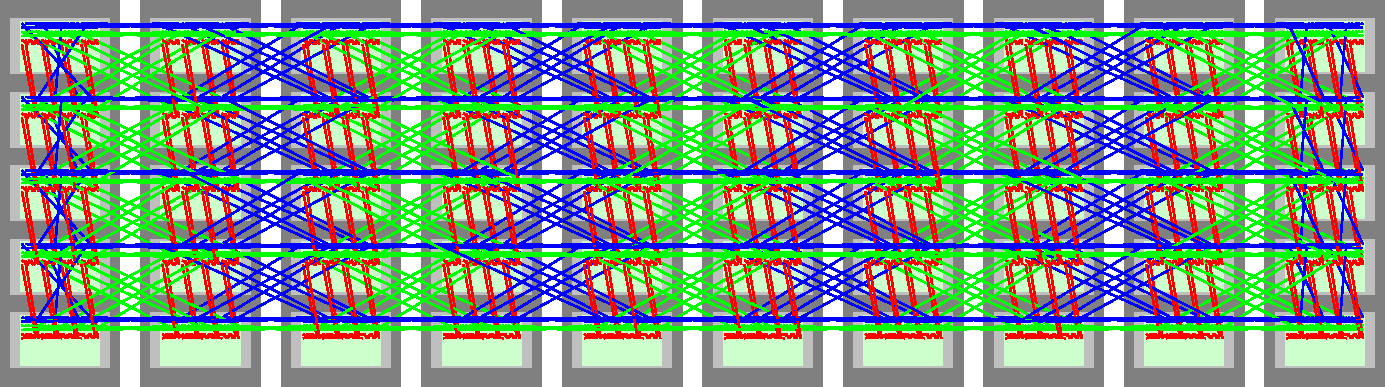
\includegraphics[width=\textwidth]{figures/spinnaker106}
			\caption{Wiring scheme for a SpiNNaker machine with 1,200 boards arranged
			in 10 cabinets. Line colour represents which of three sockets the wire is
			connected to.}
			\label{fig:spinnaker106}
		\end{figure}
	
	\subsection{Small-World Super-Computers}
	
		The connections in the brain, along with many graph-like networks observed
		in nature exhibit the `small world' property, first described by Frigyes
		Karinthy in 1929 \cite{karinthy29}. It is best known as the theory of six
		degrees of separation which states that any two randomly-selected people in
		the world are connected via a chain of no more than six acquaintances. That
		is, for a very large graph with the small-world property, only a small
		number of `hops' between nodes are required between any two places.
		
		Watts and Strogatz proposed an algorithm for generating random networks with
		the small-world property in which a regular network topology (such as a
		torus) is augmented with a small number of random connections
		\cite{watts98}. Watts-Strogatz style topologies have been shown to increase
		the bandwidth available over simple torus networks at a low additional
		wiring cost \cite{shin11}.
		
		Preliminary work has shown that latency is also improved in small-world
		networks based on tori. As a result, the latency of spikes in the system can
		be reduced potentially allowing increased simulation accuracy or speed.
		
		The work was extended to account for the wiring constraints outlined in the
		previous subsection. Even when random links requiring long cables are
		disallowed, the improvement in latency is only slightly reduced.

\section{Research Plan}

	\begin{figure}
		\center
		\begin{tikzpicture}[thick,x=0.25cm]

%%%%%%%%%%%%%%%%%%%%%%%%%%%%%%%%%%%%%%%%%%%%%%%%%%%%%%%%%%%%%%%%%%%%%%%%%%%%%%%%
% Hacked-up Gantt Library
%%%%%%%%%%%%%%%%%%%%%%%%%%%%%%%%%%%%%%%%%%%%%%%%%%%%%%%%%%%%%%%%%%%%%%%%%%%%%%%%

% An entry in the Gantt chart. Takes a label, start offset, length and slack.
% Also defines a pair of labels "[label] start" and "[label] end" which can be
% used for drawing dependency lines.
\newcommand{\ganttEntry}[4]{
	% Label
	\node (label)
				[below=1.5ex of label.south east,anchor=east,minimum height=1.7em]
				{#1}
				;
	\coordinate (gantt labels end) at (label.south east);
	
	% Box
	\draw ([shift={(#2   ,-.9ex)}]label.north east) rectangle
	      ([shift={(#2+#3,0.9ex)}]label.south east);
	
	% The tips of the box
	\coordinate (#1 end)
	         at ([shift={(#2+#3,0.9ex)}]label.south east);
	\coordinate (#1 start)
	         at ([shift={(#2   ,-.9ex)}]label.north east);
	
	% Slack line
	\draw [ultra thick]
	      ([shift={(#2+#3,0)}]$(label.north east)!0.5!(label.south east)$)
	   -- ++(#4,0);
}

\newcommand{\ganttDep}[2]{
	\draw [->,red] (#1 end) -| (#2 start);
}

\newcommand{\ganttVSep}[2]{
	\draw [#2] ([shift={(#1,0)}]gantt labels start) -- ([shift={(#1,0)}]gantt labels end);
}

% A new gantt chart. Takes a list of x-offset/label/major-label tuples. For each
% tuple a line is created with x-offset from the previous line and the span is
% labelled with "label". If major-label given, a major label will be drawn
% centered over the previous entries up until the last major-label.
\newenvironment{gantt}[1]{
	% Start the list of labels
	\node (label) [white] {Ag};
	\coordinate (gantt labels start) at (label.north east);
	\def\periods{#1}
}{
	\begin{scope}[on background layer]
		% Thick line separating from labels
		\draw (gantt labels start) -- (gantt labels end);
		
		% Start of the area covered by a "major" label
		\coordinate (gantt maj label start) at (gantt labels start);
		
		\foreach \x/\lab/\mlab in \periods {
			\coordinate (next gantt labels start) at ([shift={(\x,0)}]gantt labels start);
			\coordinate (next gantt labels end)   at ([shift={(\x,0)}]gantt labels end);
			
			% Minor label
			\node at ($(gantt labels start) !0.5! (next gantt labels start)$)
			      [anchor=west,rotate=90]
			      {\lab}
			      ;
			
			% Separator
			\ifthenelse{\equal{\mlab}{}}{
				\draw [help lines] (next gantt labels start) -- (next gantt labels end);
			}{
				\draw [help lines,thick] (next gantt labels start) -- (next gantt labels end);
			}
			
			\coordinate (gantt labels start) at (next gantt labels start);
			\coordinate (gantt labels end)   at (next gantt labels end);
			
			% Major label
			\ifthenelse{\equal{\mlab}{}}{}{
				\coordinate (next gantt maj label start) at (gantt labels start);
				\node at ($(gantt maj label start) !0.5! (next gantt maj label start)$)
				      [yshift=1cm,anchor=south]
				      {\mlab}
				      ;
				\coordinate (gantt maj label start) at (next gantt maj label start);
			}
		}
	\end{scope}
}



%%%%%%%%%%%%%%%%%%%%%%%%%%%%%%%%%%%%%%%%%%%%%%%%%%%%%%%%%%%%%%%%%%%%%%%%%%%%%%%%
% The Chart...
%%%%%%%%%%%%%%%%%%%%%%%%%%%%%%%%%%%%%%%%%%%%%%%%%%%%%%%%%%%%%%%%%%%%%%%%%%%%%%%%

\begin{gantt}{
	4/Aug/, 4/Sep/, 4/Oct/, 4/Nov/, 4/Dec/2013,%
	2/Q1/, 2/Q2/, 2/Q3/, 2/Q4/2014,%
	2/Q1/, 2/Q2/, 2/Q3/, 2/Q4/2015,%
	2/Q1/, 2/Q2/2016%
}
	\ganttEntry{SpiNNaker Modelling}          {0}{5}{3}
	\ganttEntry{Small-World SpiNNaker}        {5}{4}{1}
	\ganttEntry{Topology Comparison}          {8}{8}{4}
	\ganttEntry{Place and Routeability}       {16}{4}{0.5}
	\ganttEntry{Multicast Simulation}         {20}{1}{0.5}
	\ganttEntry{Interconnect Evaluation}      {21}{1}{0.5}
	\ganttEntry{Architecture Design}          {22}{6}{4}
	\ganttEntry{Architecture Evaluation}      {26}{4}{2}
	\ganttEntry{Thesis Writing}               {30}{8}{2}
	
	\ganttDep{SpiNNaker Modelling}{Small-World SpiNNaker};
	\ganttDep{SpiNNaker Modelling}{Topology Comparison};
	\ganttDep{SpiNNaker Modelling}{Place and Routeability};
	
	\ganttDep{Place and Routeability}{Multicast Simulation};
	
	\ganttDep{Place and Routeability}{Architecture Design};
\end{gantt}

\end{tikzpicture}

		\caption{Gantt chart of proposed research plan.  Arrows indicate
		dependencies, thick lines indicate slack.  Note non-linear scale.}
		\label{fig:plan-gantt}
	\end{figure}
	
	Initial work will focus on the development of a more detailed simulator for
	SpiNNaker's interconnect topology. This will contribute to work comparing
	actual prototype SpiNNaker hardware against various software models of its
	behaviour in collaboration with other researchers.  This work is hoped for
	journal publication later this year. This work may extend the existing INSEE
	\cite{navaridas11insee} network simulator to allow greater flexibility in
	simulated designs. Alternatively, the work may extend the simulator built as
	part of the preliminary work on SpiNNaker.
	
	With the resulting simulator, more detailed experiments will be carried out on
	the small-world topologies examined in the preliminary work. In particular,
	simulation of realistic network traffic and a more detailed model of the
	interconnect will allow better judgement of this unconventional topology.
	
	Experiments on other less common topologies, such as express cubes
	\cite{dally91} which offer latency advantages over standard torus networks,
	will be examined and compared. These experiments will follow the process
	developed during the small-world topology experiments.
	
	A further consideration when designing network topologies is the difficulty of
	assigning resources in the system. For example, when simulating a pair of
	connected neurons, they should be placed such that spikes can be quickly
	transmitted between them. In a torus-like network this typically means
	attempting to place connected neurons on chips which are near to each other.
	Though these challenges are well understood for common networks such as tori
	\cite{dally04} work will need to be done to extend this to less conventional
	networks.
	
	The penultimate stage of the project will be to carry out detailed research
	into the technologies available for implementing current interconnection
	networks. This will likely have an impact on the topology chosen as it may
	place constraints on cabling and performance as found in the preliminary
	studies of SpiNNaker.
	
	The final stage of the work will be the development of a new architecture for
	neural simulation intended specifically to improve on the SpiNNaker
	architecture. The architecture will be tested by adding further detail to the
	models developed earlier in the project. In addition, comparisons with the
	actual performance of the mature SpiNNaker hardware should be possible.

\section{Conclusion}
	
	The simulation of models of the brain has yielded promising results with high
	levels of realism being achieved. Conventional super-computer architectures
	are poorly suited to the task due to their focus on computational power rather
	than communication. This has led to the development of numerous
	special-purpose architectures for neural simulation.
	
	The SpiNNaker architecture presents an interconnection network which allows
	the system to scale-up to fit large neural models. Though well suited to
	neural simulation, preliminary work has shown that improvements may be
	possible through the use of alternative network topologies. In addition, tools
	have been developed which will enable the performance and practicality of new
	interconnection topologies to be evaluated.
	
	The project will eventually develop a new architecture for neural simulation
	with a focus on the topology of the interconnection network. Work will develop
	from the preliminary studies of SpiNNaker with the construction of a flexible
	network simulator which will allow new topologies to be tested and evaluated.
